% !TEX root = ./arock_pkg_main.tex
\section{Architecture}

ARock reduces each application to the fixed-point problem \eqref{eqn:fix_point_set} 
\begin{equation}\label{eqn:fix_point_set}
\text{find } x \text{ such that } x = \cT x
\end{equation}
with the fixed-point operator $\cT$ being CF. The operator $\cT$ can be a single stand along operator or formed by a combination of multiple CF operators. Then the ARock kernel takes the operator $\cT$ and runs the coordinate update algorithm with a given number of workers. Figure \ref{fig:arch} gives an overview of the multilevel architecture of the ARock package. In the following subsections, we explain each of the levels in more details. 
\begin{figure}[!h]
      \centering
        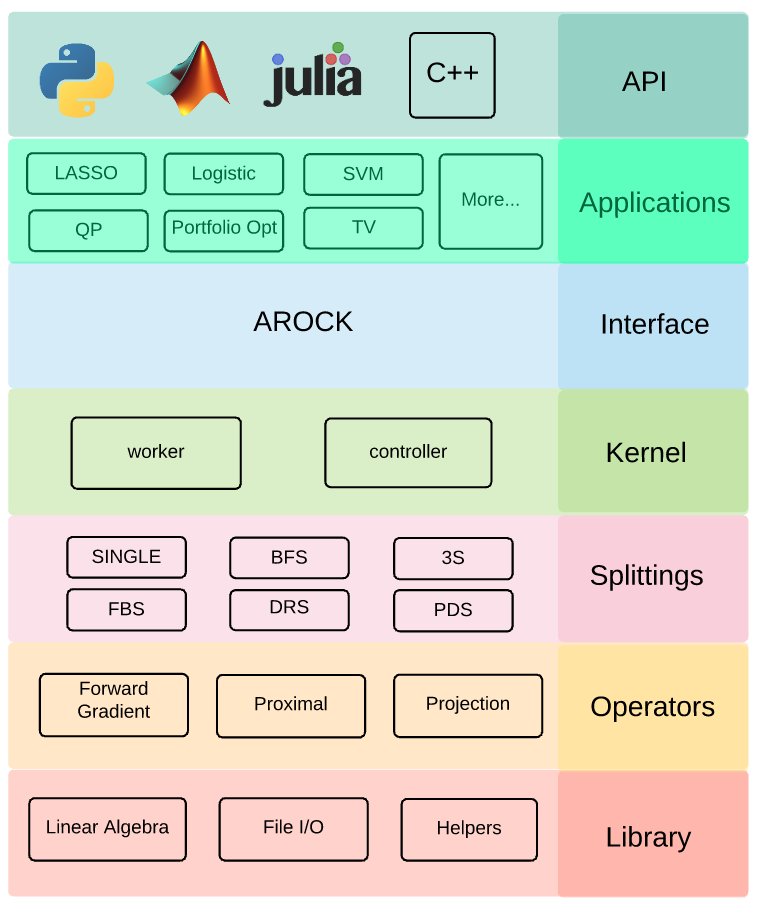
\includegraphics[width=0.45\textwidth]{./figs/architecture.png}
      \caption{Architectures for distributed memory systems. Linear algebra serves as the foundation for ARock. Other layers are structured according to the discussions in Section ??.}
        \label{fig:arch}
\end{figure}


\subsection{Library}
The library layer includes three major components: data structures and linear algebra functions, file I/O functions, and helper functions. The primary data structures are dense vector, dense matrix and sparse matrix. We implemented a few handy BLAS (Basic Linear Algebra Subprograms) wrappers. File I/O functions for matrices in the matrix market format\footnote{\url{http://math.nist.gov/MatrixMarket/formats.html}} and LIBSVM format\footnote{\url{https://www.csie.ntu.edu.tw/~cjlin/libsvmtools/datasets/}} are also implemented. Helper functions include a list of objective functions, command-line argument parsers, and error handling functions. Those functions are extensively used in the operator layer and the splitting layer. 

\subsection{Operators}
The operator layer is a library of projection operators, proximal operators and forward operators which are useful for high-level iterative algorithms. Currently, we implemented 17 operators. These operators are modularized and implemented in the form of \emph{function object (functor)}. 

In general, each operator struct has three overloaded parenthesis operators: one consumes a scalar and calculates the update; one takes a vector and an index then applies the coordinate update; one takes an input vector and an output vector, then performs full update to the input vector and saves the results in the output vector. Constructors and update cached variable function are also provided. If an operator involves data, pointers to the data are added as member variables. The following code is a template for implementing operators.
\begin{lstlisting}[language=C++]
struct operator_name {
  double step_size;  // operator related step size
  double weight;  // weight on the operator  
  double operator() (double val);  // scalar update operator  
  // coordinate update operator
  double operator() (Vector* v, int index = 0);  
  // full update operator
  void operator() (Vector* v_in, Vector* v_out); 
  // update cached variables
  void update_cache_vars(double old_x_i, double new_x_i, int i);
  operator_name();  // default constructor
  operator_name(argument list);  // customized constructor
};
\end{lstlisting}


\cut{
\begin{lstlisting}[language=c++]
  struct functor_name {
    // the step_size that associated with the operator  
    double step_size;
    // weight on the original function, e.g., f(x) = weight ||x||_1
    double weight;      
    // returns the operator evaluated on v at the given index
    double operator() (Vector* v, int index);
    // returns the operator evaluated on v at the given index
    double operator() (double val, int index);
    // full update
    void operator() (Vector* v_in, Vector* v_out);
    // (Optional) update the cached variables, it 
    // takes the old x_i and new x_i, updated at index.
    void update_cache_vars (double old_x_i, double new_x_i, int index);
    // update the step size. The step size might be
    // changed during the iterative process
    void update_step_size (double step_size_) {
      step_size = step_size_;
    }
    // customized constructor
    functor_name (double step_size_, double weight_ = 1.) :
        step_size(step_size_), weight(weight_) {}
    // default constructor
    functor_name () : step_size(0.), weight(1.) {}
  };
\end{lstlisting}
}

\subsection{Splitting Schemes}
Splitting schemes are templated on operators. Based on the discussions in Section \ref{sec:splitting}, we implemented several splitting schemes, including PPA, FBS, BFS and PRS. The structure of the splitting scheme has the following form. 
 \begin{lstlisting}[language=c++]
 template <typename Op1, typename Op2, ...>
 struct OperatorSplitting {
   double relaxation_step_size; 
   Vector* x;
   Op1 p1;  // define the operators
   // calculates the update of x at index
   double operator(int index);
   // update the operator related parameters
   void update_params(Params* params);
   // customized constructor
   OperatorSplitting(argument list);
};
\end{lstlisting}
It usually has one or more than one operators as the template arguments. It has an overloaded parenthesis operator which performs updates to the unknown variable $x$ and maintained variables. The update is carried out by calling appropriate member functions of the templated operators. An example of the implementation of the parenthesis operator for FBS is shown below. 
\begin{lstlisting}[language=c++]
  double operator() (int index) {
    // Step 1: read the old x[index]
    double old_x_at_idx = (*x)[index]; 
    // Step 2: local calculation
    double forward_grad_at_idx = forward(x, index);
    double val = backward(forward_grad_at_idx);
    double S_i = old_x_at_idx - val;
    // Step 3: get the most recent x[index] before updating it
    old_x_at_idx = (*x)[index];
    // Step 4: update x at index 
    (*x)[index] -= relaxation_step_size * S_i;    
    // Step 5: update the maintained variable Atx
    forward.update_cache_vars(old_x_at_idx, (*x)[index], index);
    return S_i;
  }
\end{lstlisting}



\subsection{Worker and Controller}
ARock consists of several workers and a controller. Each worker has access to the shared data, the maintained variables, the unknown parameter $x$, and other algorithm related constants. Each worker continuously updates some coordinates of $x$ until the stopping criterions are satisfied. The coordinates can be updated in a cyclic or random fashion. At the same time, workers share delay monitoring information and convergence progress information with the controller, who use the information to dynamically update the step sizes to facilitate the convergence of ARock. Figure~\ref{fig:worker_controller} demonstrates the relations of workers, controller, and shared memory.  
\begin{figure}[!h]
      \centering
        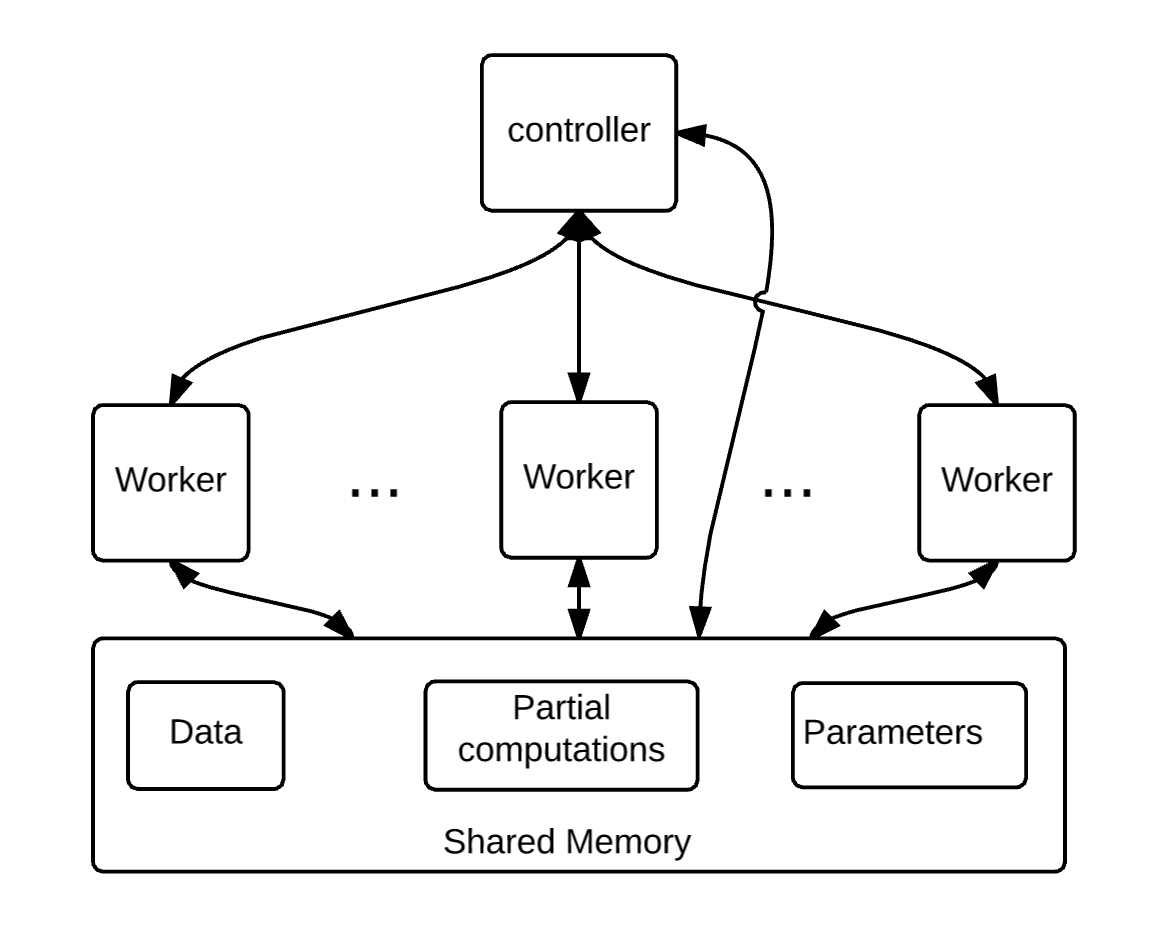
\includegraphics[width=0.5\textwidth]{./figs/worker_controller.png}
      \caption{Relationship between workers, controller and shared memory.}
        \label{fig:worker_controller}
\end{figure}

\subsection{ARock Interface}
The ARock interface simply spawns a set of threads with one thread taking the controller role and the rest of threads being the workers. The interface of ARock is the following. It takes three inputs, including a splitting scheme, a parameter structure and a controller.
\begin{lstlisting}[language=c++]
template<typename Splitting>
void AROCK(Splitting op, Params parameters, Controller<Splitting> controller);
\end{lstlisting}


\subsection{Applications}
Section \ref{sec:quick_start} gives an example of using ARock to solve the sparse logistic regression problem. Other applications are implemented or can be implemented similarly. We have implemented several applications from statistical machine learning and scientific computing with the ARock framework. The applications can be compiled into executable files, which can then be executed through the command-line interface. For an unimplemented application, if the necessary operators and splitting schemes are defined in the ARock library, then creating an async-parallel algorithm can be as simple as calling ARock on the appropriate splitting scheme. 


